%%%%%%%%%%%%%%%%%%%%%%%%%%%%%%%%%%%%%%%%%%%%%%%%%%%%%%%%%%%%%%%%%%%%%
%
% talk intro optimization Cotonou 2022
%
%%%%%%%%%%%%%%%%%%%%%%%%%%%%%%%%%%%%%%%%%%%%%%%%%%%%%%%%%%%%%%%%%%%%%

\documentclass[12pt]{beamer}
\usepackage[utf8]{inputenc}
\usepackage{amsmath}
\usepackage{amsfonts}
\usepackage{amssymb}
\usepackage{graphicx}
\graphicspath{{figures/}{Figures/}}
%\usepackage{beamerthemesplit}
%\usepackage{beamerthemeshadow} 
\usepackage{color}
\usepackage{hyperref}
\usepackage{xspace}
\usepackage{xifthen}
\usepackage{multicol}
\usepackage{mathtools}
\usepackage{algorithm,algorithmicx}
\usepackage{algcompatible}
\usepackage{bbm}
\usepackage{textcomp}
\usepackage{yfonts}

\usepackage{tikz}
\usetikzlibrary{calc,shapes,arrows}

% custom commands in sty file, for easier writting and change of notations
\usepackage{my_notations}
\newcommand*{\mmds}{\enm{\text{MMD}^2}}

\usetheme{Madrid}
\usecolortheme{beaver}

%%%%%%%%%%%%%%%%%%%%%%%%%%%%%%%%%%%%%%%%%%%%%%%%%%%%%%%%%%%%%%%%%%%%%
\begin{document}
\title
[Optimization: multi-tasker or utopia?
\hspace{0.1cm}
\insertframenumber/\inserttotalframenumber]
{Optimization for quantitative decisions: a versatile multi-tasker or an utopia?}
\author
[R. Le Riche]
{\large Rodolphe Le Riche$^{*}$}
\institute[CNRS LIMOS]{$^*$~CNRS at LIMOS (Mines Saint Etienne, UCA) France
} 
\date[July 2022]{25 July 2022 \\
Cotonou, Benin, IA summer school 
\\\vskip\baselineskip
{\small Acknowledgements : Vallet fundation}
} 
\begin{frame}
\titlepage
\end{frame}

%=======================================================================================
%\begin{frame}[allowframebreaks]
%\frametitle{Content} 
%\begin{multicols}{2}
%\tableofcontents[currentsection]
%\end{multicols}
%\end{frame}


%=======================================================================================
\begin{frame}[allowframebreaks]
\frametitle{The advent of optimization algorithms}
\begin{minipage}[b]{0.25\textwidth}
\centering
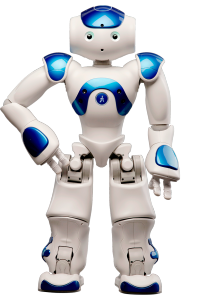
\includegraphics[width=0.4\textwidth]{Figures/NAO.png}
\\ ``Intelligence'' =
\end{minipage} 
\hfill
\begin{minipage}[b]{0.2\textwidth}
{\scriptsize \cite{bachoptimization}}
\vskip 2cm
~
\end{minipage} 
\\
\hfill
\begin{minipage}[t]{0.2\textwidth}
\centering
 models + 
\\
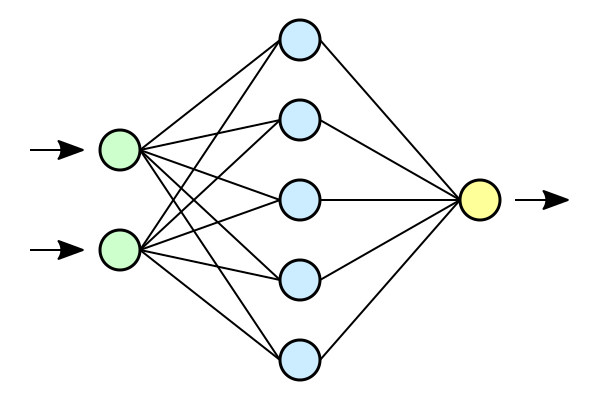
\includegraphics[width=\textwidth]{Figures/neural_network.png} 
\end{minipage} 
\begin{minipage}[t]{0.2\textwidth}
\centering
\textbf{\textcolor{red}{algorithms}} + 
\\
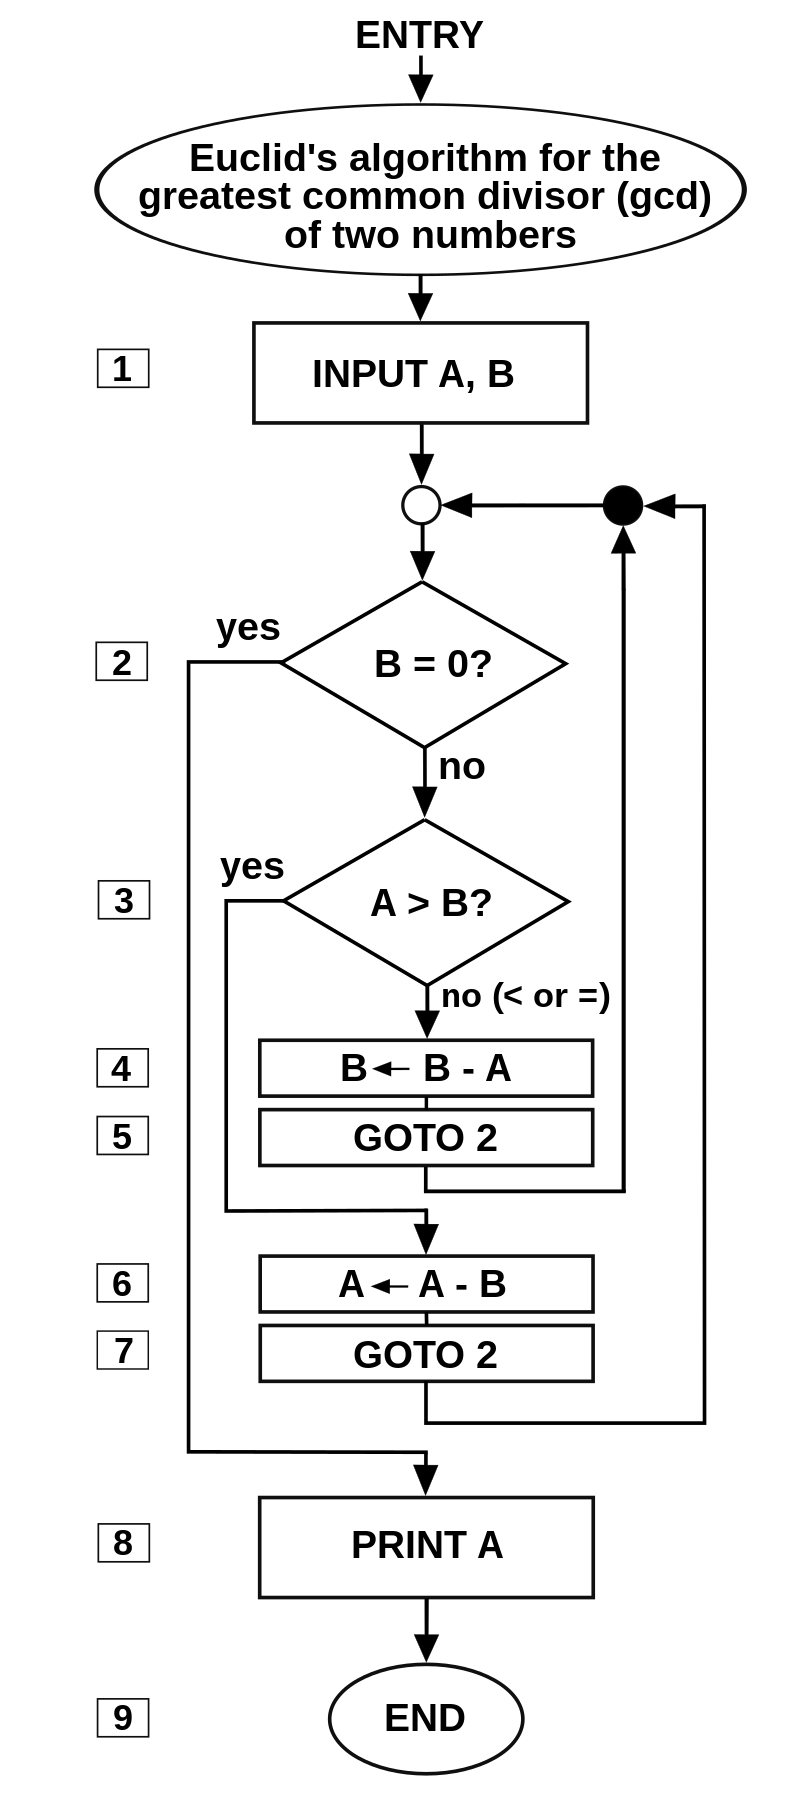
\includegraphics[width=0.5\textwidth]{Figures/algorithm.png} 
\end{minipage} 
\begin{minipage}[t]{0.2\textwidth}
\centering
data + 
\\\vskip 0.2cm

\includegraphics[width=\textwidth]{Figures/data.png} 
\end{minipage} 
\begin{minipage}[t]{0.2\textwidth}
\centering
computing power 
\\\vskip 0.2cm
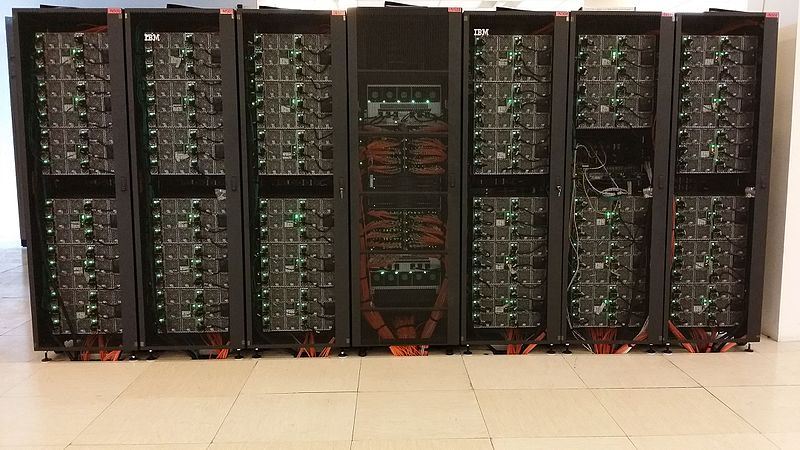
\includegraphics[width=\textwidth]{Figures/supercomputer.jpg} 
\end{minipage} 
\newpage
There are numerous conferences$^\star$ (and journals) where new optimization algorithms are presented, whether in 
\begin{itemize}
\item applied mathematics. Ex: {\scriptsize SIAM Conf. on Optimization, FGS (French-German-Swiss) workshops series, PGMO Days, \ldots}
\item computer science (including machine learning). Ex: {\scriptsize LION (Learning and Intelligent OptimizatioN conf.), EURO (EURopean Operational research soc.) conf., Optimization days, NEURIPS, \ldots}
\item or in application fields. Ex: {\scriptsize SIAM Conf. on Uncertainty Quantification (statistics), AIAA/MAO (Multidisciplinary Analysis and Optimization) or WCSMO (World Congress on Structural and Multidisciplinary Optimization) conferences (engineering), ECCOMAS (aeronautics), ICASP (civil engineering), \ldots}
\end{itemize}
\hfill($^\star$ {\scriptsize : arbitrarily listing some of the meetings I participated to} )
\newpage
Some recent algorithms are highly cited, i.e., are seen as key technological components : 
\begin{itemize}
\item NAG (\cite{nesterov1983method}, 1983, $>5500$ citations),
\item CMA-ES (\cite{hansen2001completely}, 2001, $>4100$ citations),
\item ADAGRAD (\cite{duchi2011adaptive}, 2011, $>10400$ citations),
\item RMSprop (\cite{tieleman2012lecture}, 2012, $>6000$ citations),
\item Adam (\cite{kingma2014adam}, 2014, $>113000$ citations),
\item \ldots
\end{itemize}
\end{frame}


%=======================================================================================
\begin{frame}
\frametitle{}
\centering
{\usebeamerfont*{frametitle}\usebeamercolor[fg]{frametitle} 
Optimization algorithms? 
\vskip\baselineskip
What are we talking about?
}
\end{frame}

%%%%%%%%%%%%%%%%%%%%%%%%%%%%%%%%%%%%%%%%%%%%%%%%%%%%%%%%%%%%%%%%%%
\begin{frame}[allowframebreaks]
\frametitle{The fundamental optimization problem}
\begin{minipage}{\textwidth}
\begin{minipage}{0.5\textwidth}
\centering
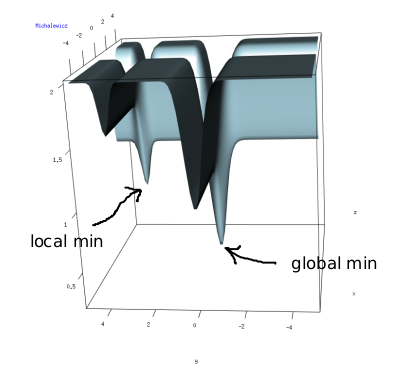
\includegraphics[width=0.9\textwidth]{michalewicz_local_global.png} \\
\vspace{-0.4cm}
{\small (2D continuous example)}
\end{minipage}
\begin{minipage}{0.45\textwidth}
Find the lowest point of a function,
\begin{equation*}
\min_{x \in \mathcal S } f(x)
\end{equation*}
\end{minipage}
\vskip\baselineskip
Looks easy on this drawing. \\
But the function is known pointwise, each evaluation costs computer time, and $\mathcal S$ may be complex (high-dimensional, non-continuous, constrained \ldots)
\end{minipage}
\newpage
\begin{minipage}{0.45\textwidth}
\centering
\begin{tikzpicture}
\node[anchor=south west,inner sep=0, outer sep=0] (contour) at (0,0) {
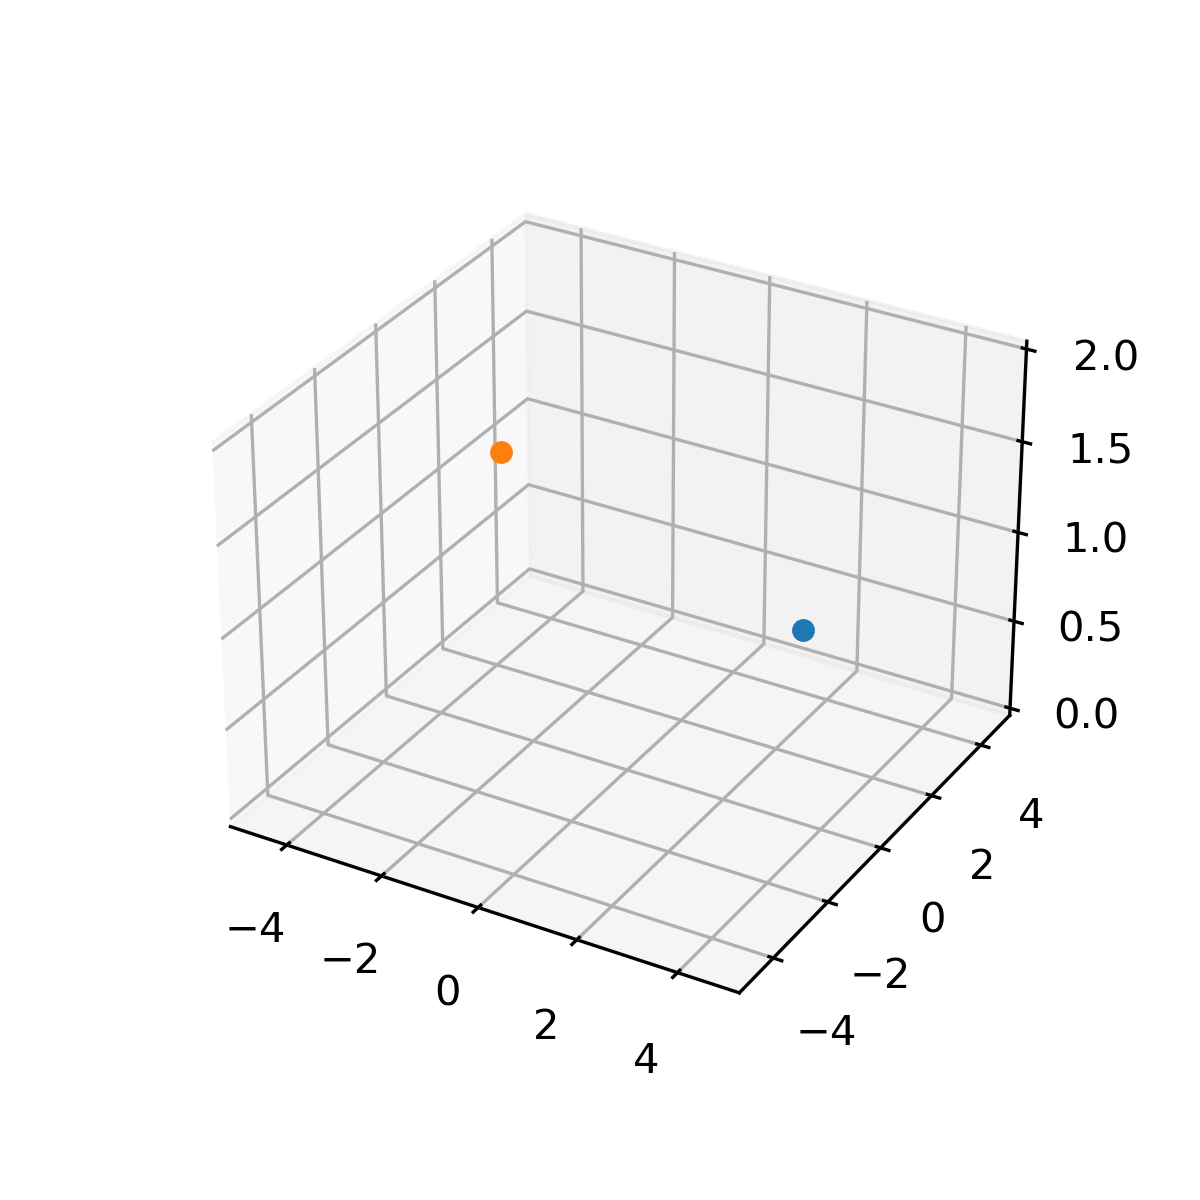
\includegraphics[width=0.9\textwidth]{two_3D_points.png}
};
\begin{scope}[x={(contour.south east)},y={(contour.north west)}]
%\draw[help lines,xstep=0.1,ystep=0.1] (0,0) grid (1,1);
\node[] (xstar) at (0.73,0.5) {$\widehat{x^\star}$};
\node[] (xprime) at (0.37,0.65) {$x'$};
\end{scope}
\end{tikzpicture}
\vspace{-0.4cm}
{\small (what the random optimizer sees)}
\end{minipage}
\hfill
\begin{minipage}{0.45\textwidth}
Random search \hfill ~\\
\noindent\rule{\textwidth}{1pt}
{\scriptsize
\begin{algorithmic}%[1]
\REQUIRE $x^\text{LB},~x^\text{UB},t^\text{max}$
\STATEx $t \leftarrow 0,~\widehat{f^\star} \leftarrow + \infty$
\WHILE{$t<t^\text{max}$}
\STATE $x' \leftarrow \mathcal U[x^\text{LB},~x^\text{UB}]\quad$ \COMMENT{uniform law}
\STATE calculate $f(x')$, $t \leftarrow t+1$
\IF{$f(x')<\widehat{f^\star}$}
\STATE $\widehat{x^\star}\leftarrow x' \quad,\quad \widehat{f^\star} \leftarrow f(x')$
\ENDIF
\ENDWHILE
\STATE \textbf{return} $\widehat{x^\star}, \widehat{f^\star}$
\end{algorithmic}
}
\vspace{-0.8\baselineskip}
\noindent\rule{\textwidth}{1pt}
\end{minipage}
\end{frame}


%%%%%%%%%%%%%%%%%%%%%%%%%%%%%%%%%%%%%%%%%%%%%%%%%%%%%%%%%%%%%%%%%
\begin{frame}
\frametitle{Optimization = a quantitative formulation of decision}
Optimization is a way of mathematically modeling decision.
\vskip\baselineskip
\mbox{
\begin{minipage}[c]{0.3\textwidth}

\includegraphics[width=\textwidth]{decision-clipart.jpg}
\end{minipage}
\begin{minipage}[c]{0.7\textwidth}
\begin{equation*}
\min_{x \in \mathcal S} f(x)
\end{equation*}
\begin{itemize}
\item $x$ vector of decision parameters (variables)~: dimensions, investment, tuning of a machine / program, \ldots
\item $f(x)$~: decision cost, minus $\times$ performance, \ldots 
\item $\mathcal S$~: set of possible values for $x$, search space
\end{itemize}
\end{minipage}
} % end mbox
Don't forget the human in the loop ! in \cite{tsoukias2008decision}, broader framework (model of the human rationality) $\Rightarrow$ decision \alert{aiding} theory.
\\
Here, modest goal : optimization as a \alert{tool}.
\end{frame}


\section{Bibliography}

%=======================================================================================
\begin{frame}[allowframebreaks]
\frametitle{References}
\scriptsize
%\vspace{-1.cm}
%\setbeamertemplate{bibliography item}{[\theenumiv]} % to have numbers in biblio with beamer
%   \bibliographystyle{plain}
   \bibliographystyle{apalike}
   \bibliography{biblio}
\end{frame}

\end{document}

